The signal is modelled using simulated events. In this version of the note,
we present the same BDT outputs used in the 2015 analysis. The generator-level
information is identical to the 2015 samples, thus little change is expected.
The plots in this section will be udpated to reflect BDT output with 2016 samples
in later versions of this note. The simulation has two
different sources of systematic uncertainty. The first source of
uncertainty is correction factors applied to the simulation in
order to better reproduce the detector conditions and performance in
data. The second source is assumptions made in the theoretical
models that were used to produce the simulation. We account for
uncertainties from both sources.

\subsection{Correction factors and experimental uncertainties}

As discussed in Section~\ref{sec:objects}, we use scale factors to
correct for differences in lepton performance between data and
simulation. The scale factors account for the differences
in the trigger, lepton Loose and Tight selections.
Each of these scale factors has an uncertainty associated
with it as discussed in that section, and it's propagated in the final
uncertainties on signal yields.\\

%The corrections that we apply to jet energies in simulation have
%uncertainties associated with them~\cite{cmsJEC}. The uncertainties
%are parameterised as a function of $\pt$, $\eta$. We assess the impact of the uncertainties by shifting the jet
%energy correction factors for each jet up and down by $\pm1\sigma$ and
%re-calculating all kinematic quantities. The effect on the shape of
%the BDT discriminators used in the signal extraction is shown in Fig.~\ref{fig:JEConBDTshape}.
%Systematic effects both on normalization and shape are taken into account in extracting the
%results. 

%\begin{figure}[htb]
%	\centering 
%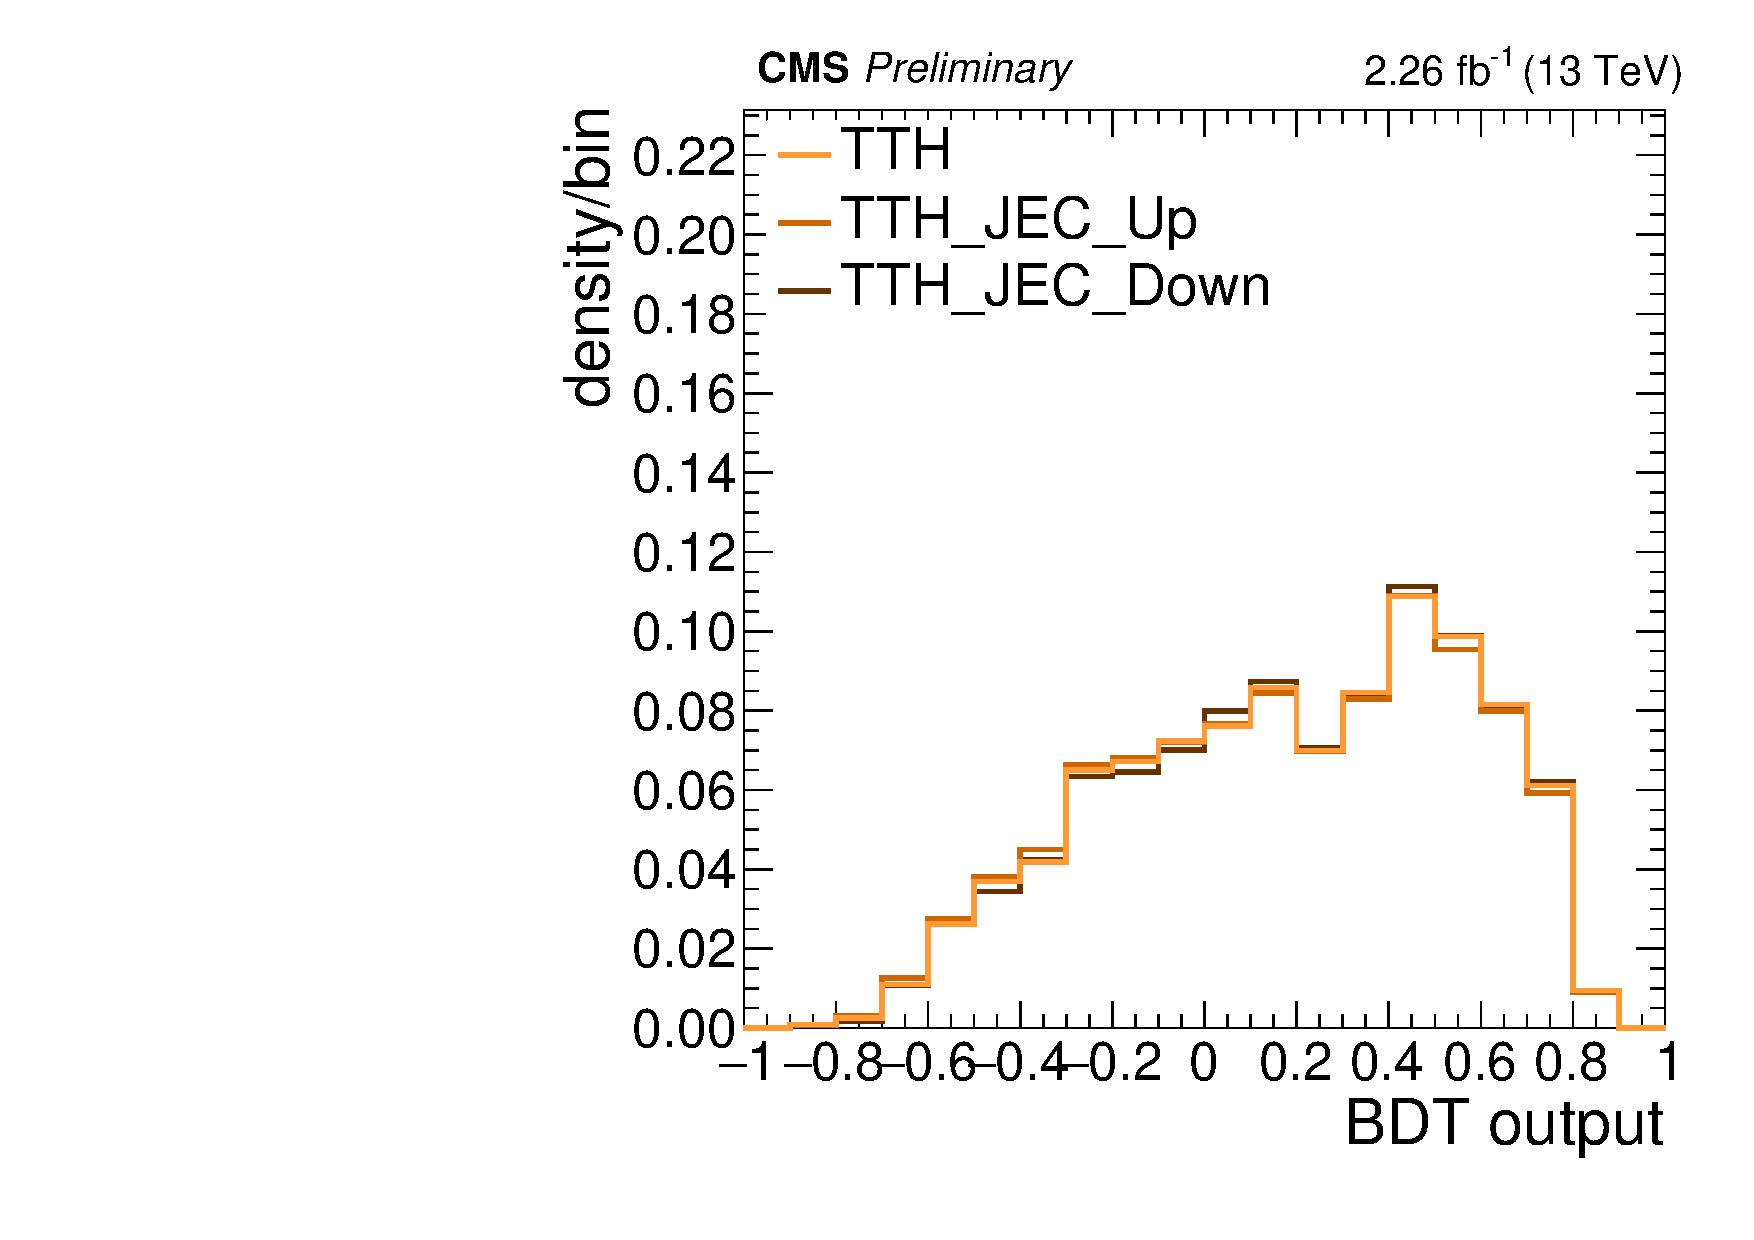
\includegraphics[width=0.35\textwidth]{plots_signal/exp_uncert/2lss/JEC_ttH/kinMVA_2lss_ttbar}
%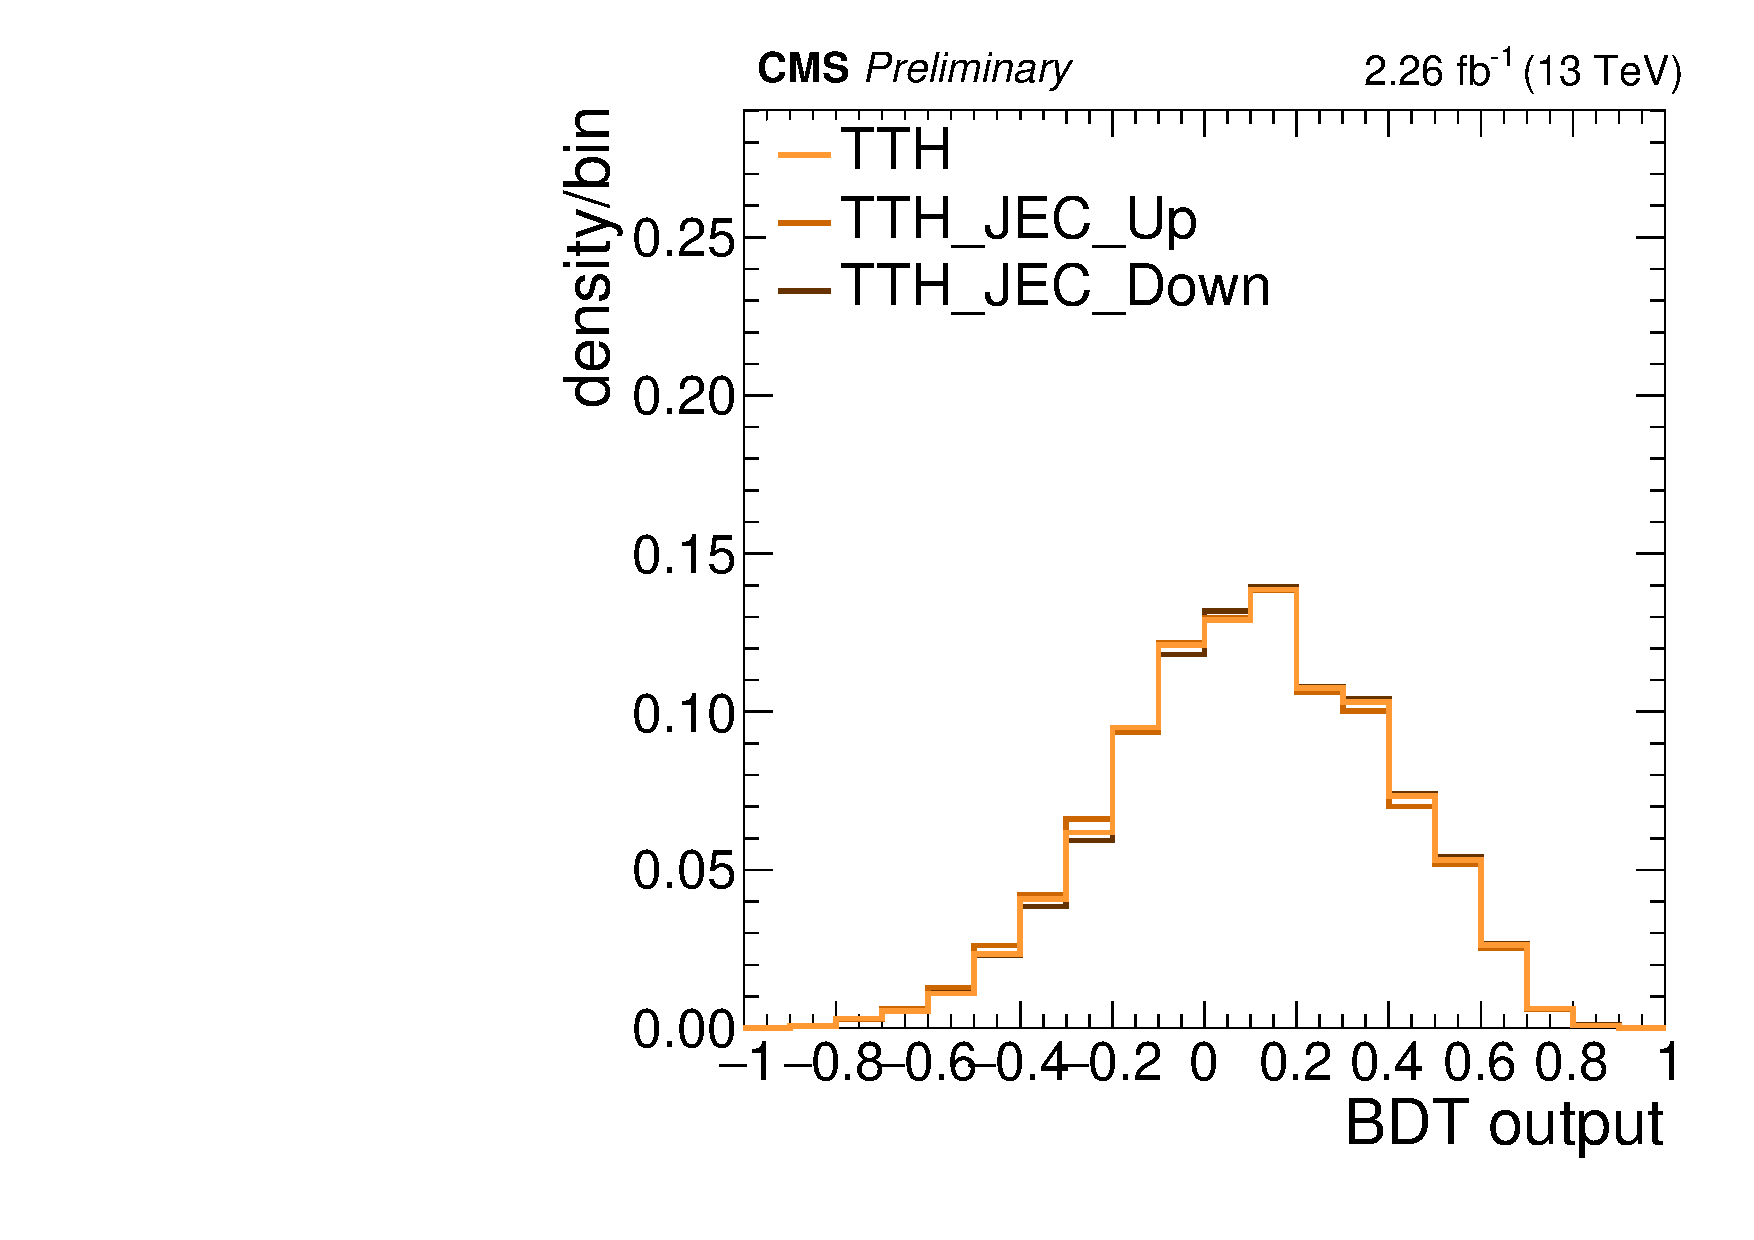
\includegraphics[width=0.35\textwidth]{plots_signal/exp_uncert/2lss/JEC_ttH/kinMVA_2lss_ttV}
%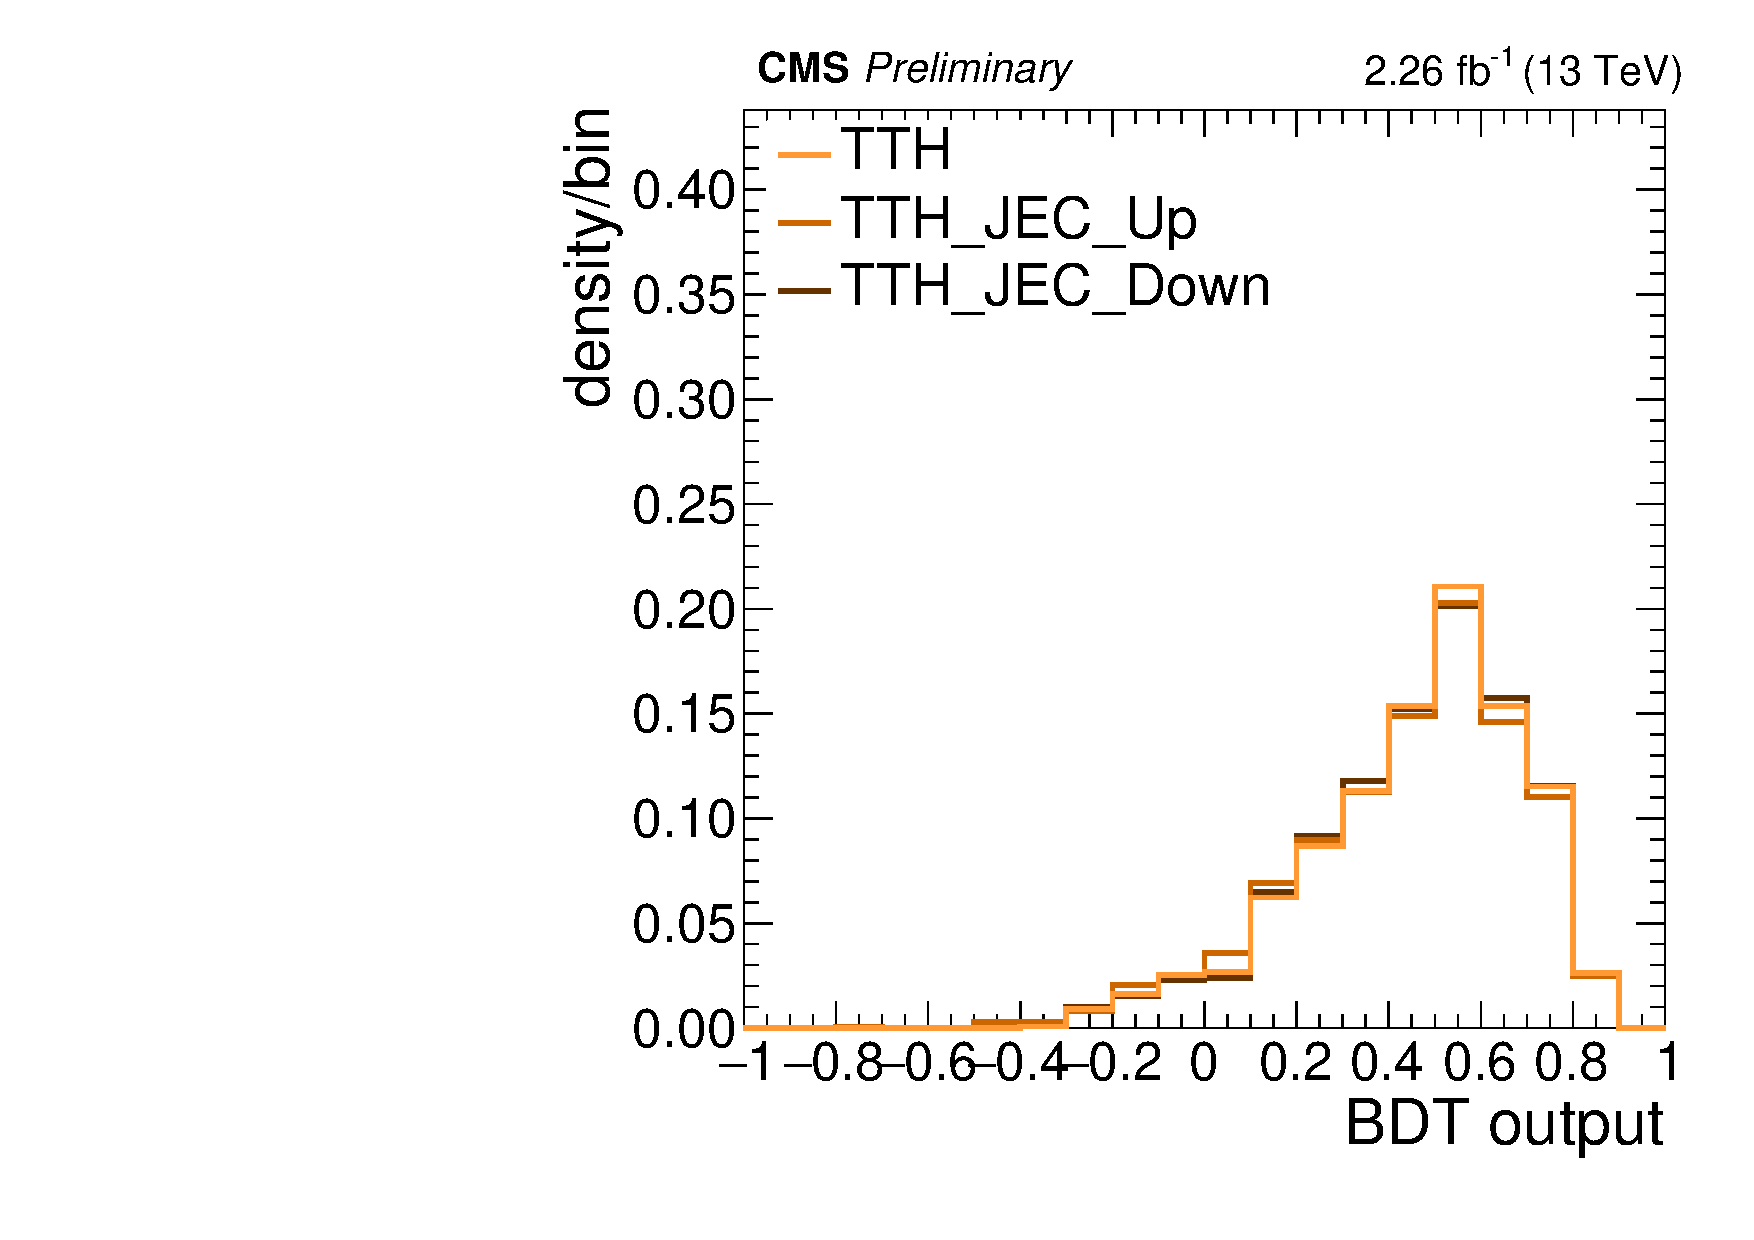
\includegraphics[width=0.35\textwidth]{plots_signal/exp_uncert/3l/JEC_ttH/kinMVA_3l_ttbar}
%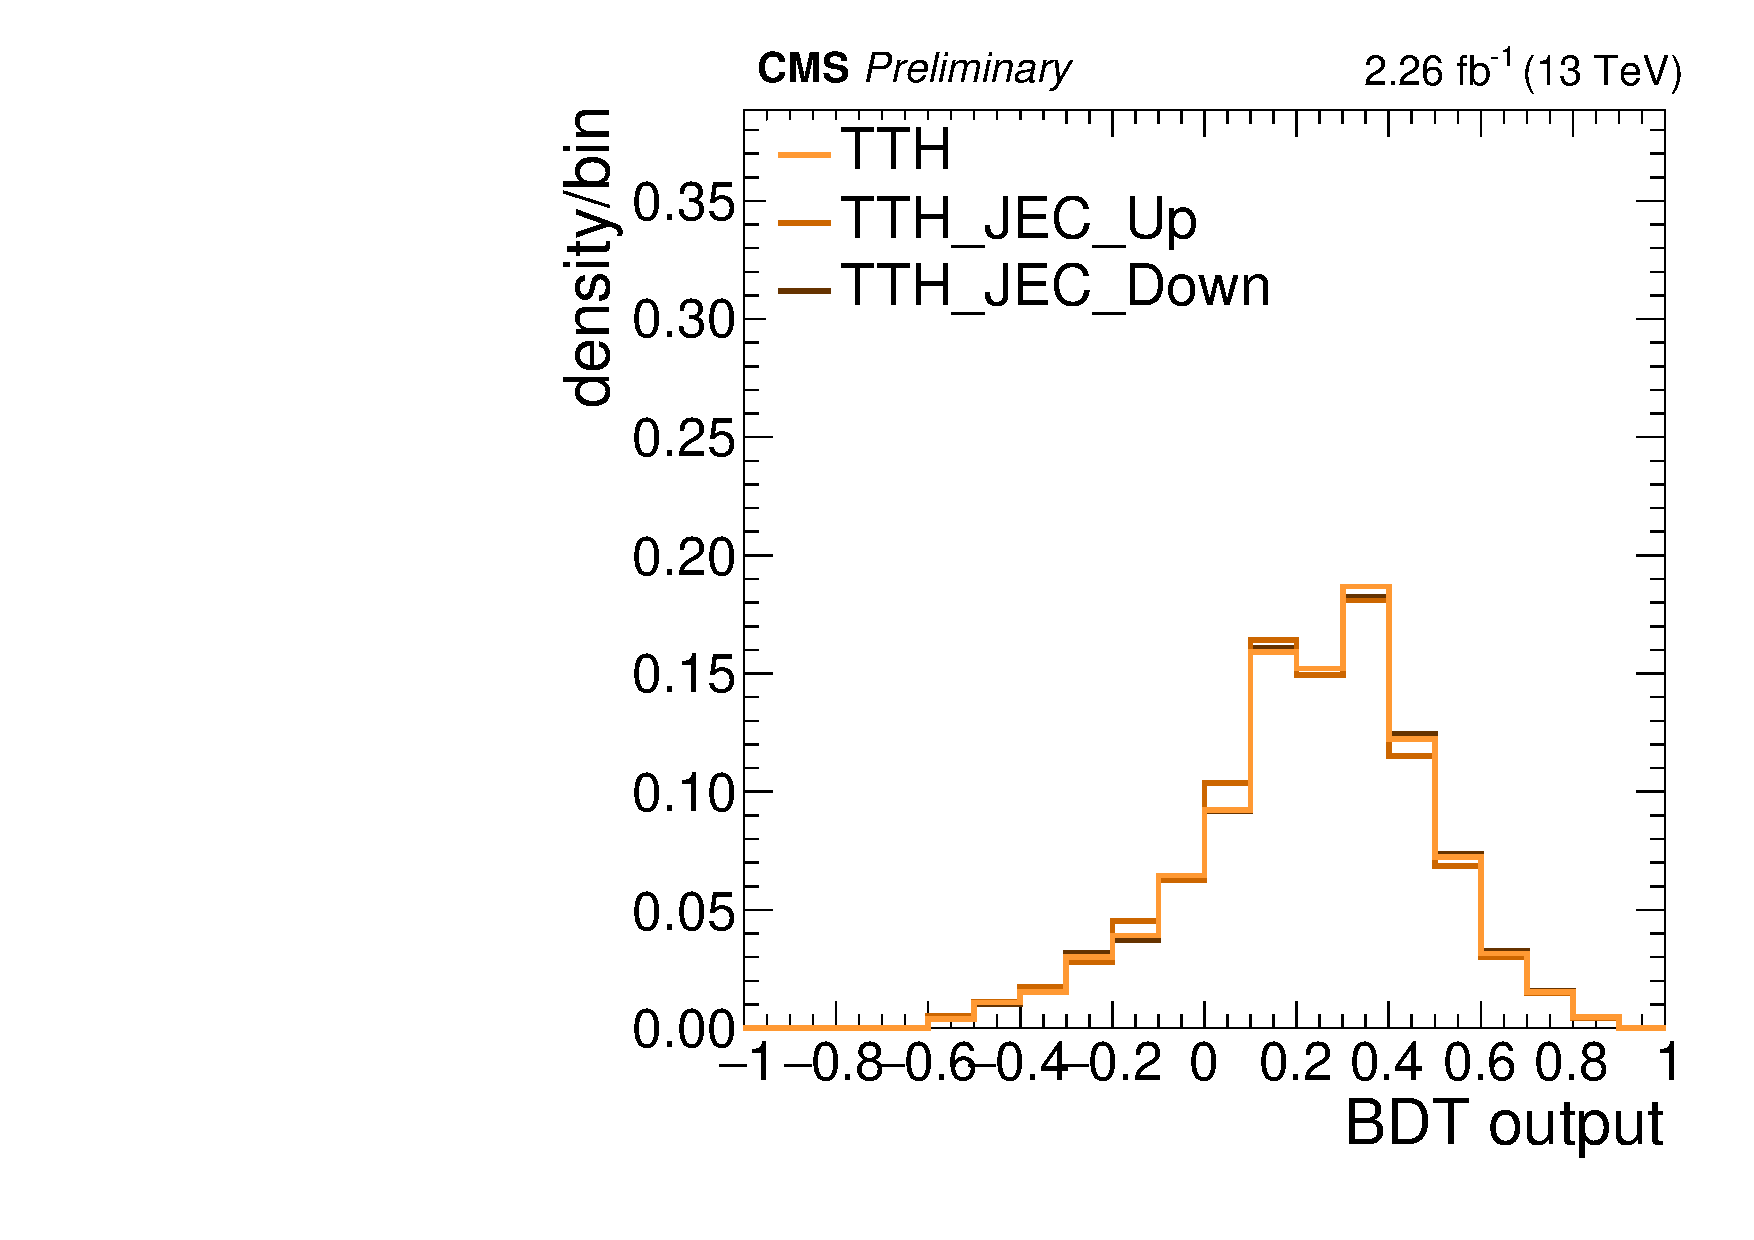
\includegraphics[width=0.35\textwidth]{plots_signal/exp_uncert/3l/JEC_ttH/kinMVA_3l_ttV}
%	\caption{The BDT output distribution of the ttH signal, shown for the training against ttbar 
%	(left) and ttV (right) in the two same sign leptons (upper) and three lepton (lower) final state,
%	 with the jet energy scale variations of one standard deviation included in order to estimate 
%	 the shape uncertainties.}
%	\label{fig:JEConBDTshape}
%\end{figure}

In the RunI analysis we found that the uncertainty from the jet energy resolution plays a
negligible role in this analysis.

%% There is also an uncertainty associated with the jet energy
%% resolution. This uncertainty is small even for analyses where jets
%% play a central role. For instance, the $\ttH$, $\PH\to\bbbar$ analysis
%% is more sensitive to jets effects than this
%% analysis~\cite{cms_tthbb_summer13}. It found that the uncertainty
%% from the jet energy resolution was small effect.  We have assumed that
%% the impact is also small for our analysis.

The uncertainties on the correction for the data/sim differences in the b-tagging
performance described in~\ref{sec:objects}  are
parameterised as a function of $\pt$, $\eta$, and jet flavor. We assess their effect on the analysis by shifting the weight of
each jet up and down by $\pm1\sigma$ of the appropriate uncertainty
and recalculating the overall event weight. 


\subsection{Theoretical uncertainties}

\textcolor{red}{We are completing the update of the impact of theoretical uncertainties on the signal prediction, it will be included in the next update of the AN.}

The theoretical uncertainties on the NLO prediction for the inclusive $\ttH$ production cross section
amount to $+5.8$$-9.2\%$ from unknown higher orders in the perturbative series and $3.6\%$ from the knowledge
of the parton distribution functions (PDFs) and $\alpha_{s}$ ~\cite{YR4}. These uncertainties are propagated to the
final normalization of the signal yields. \\
In addition to the overall normalisation, systematic uncertainties of theoretical origin on the
distribution of the events in the final discriminating variables are considered, estimated
conventionally by varying the normalisation and factorisation scales up and down by a factor of two and
matching threshold between matrix element and parton shower (Fig.~\ref{fig:ScaleonBDTshape}).
In the current version of the results the shape uncertainties on the BDTs output are of the order of $2\%$ to $3\%$.

\begin{figure}[htb]
	\centering 
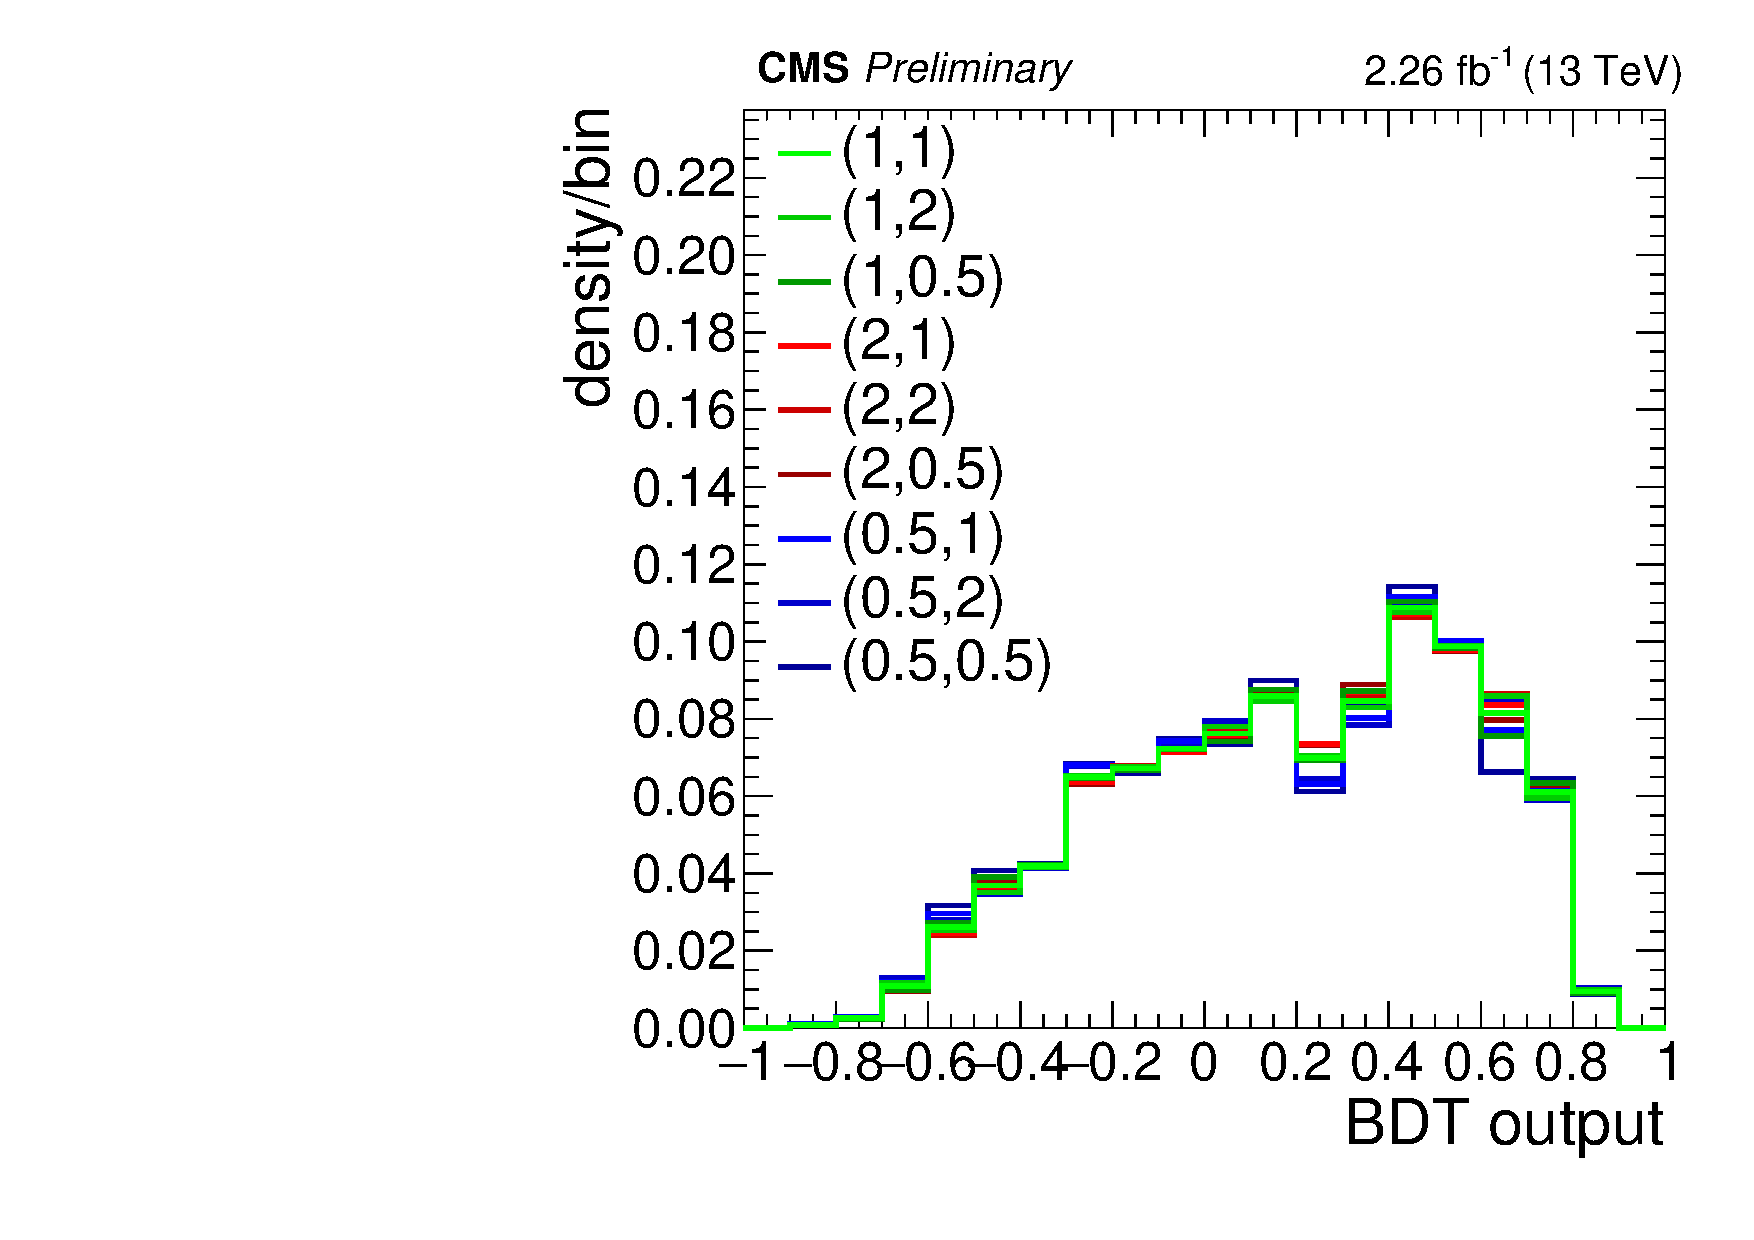
\includegraphics[width=0.35\textwidth]{plots_signal/theor_uncert/2lss/muR_muF_ttH/kinMVA_2lss_ttbar}
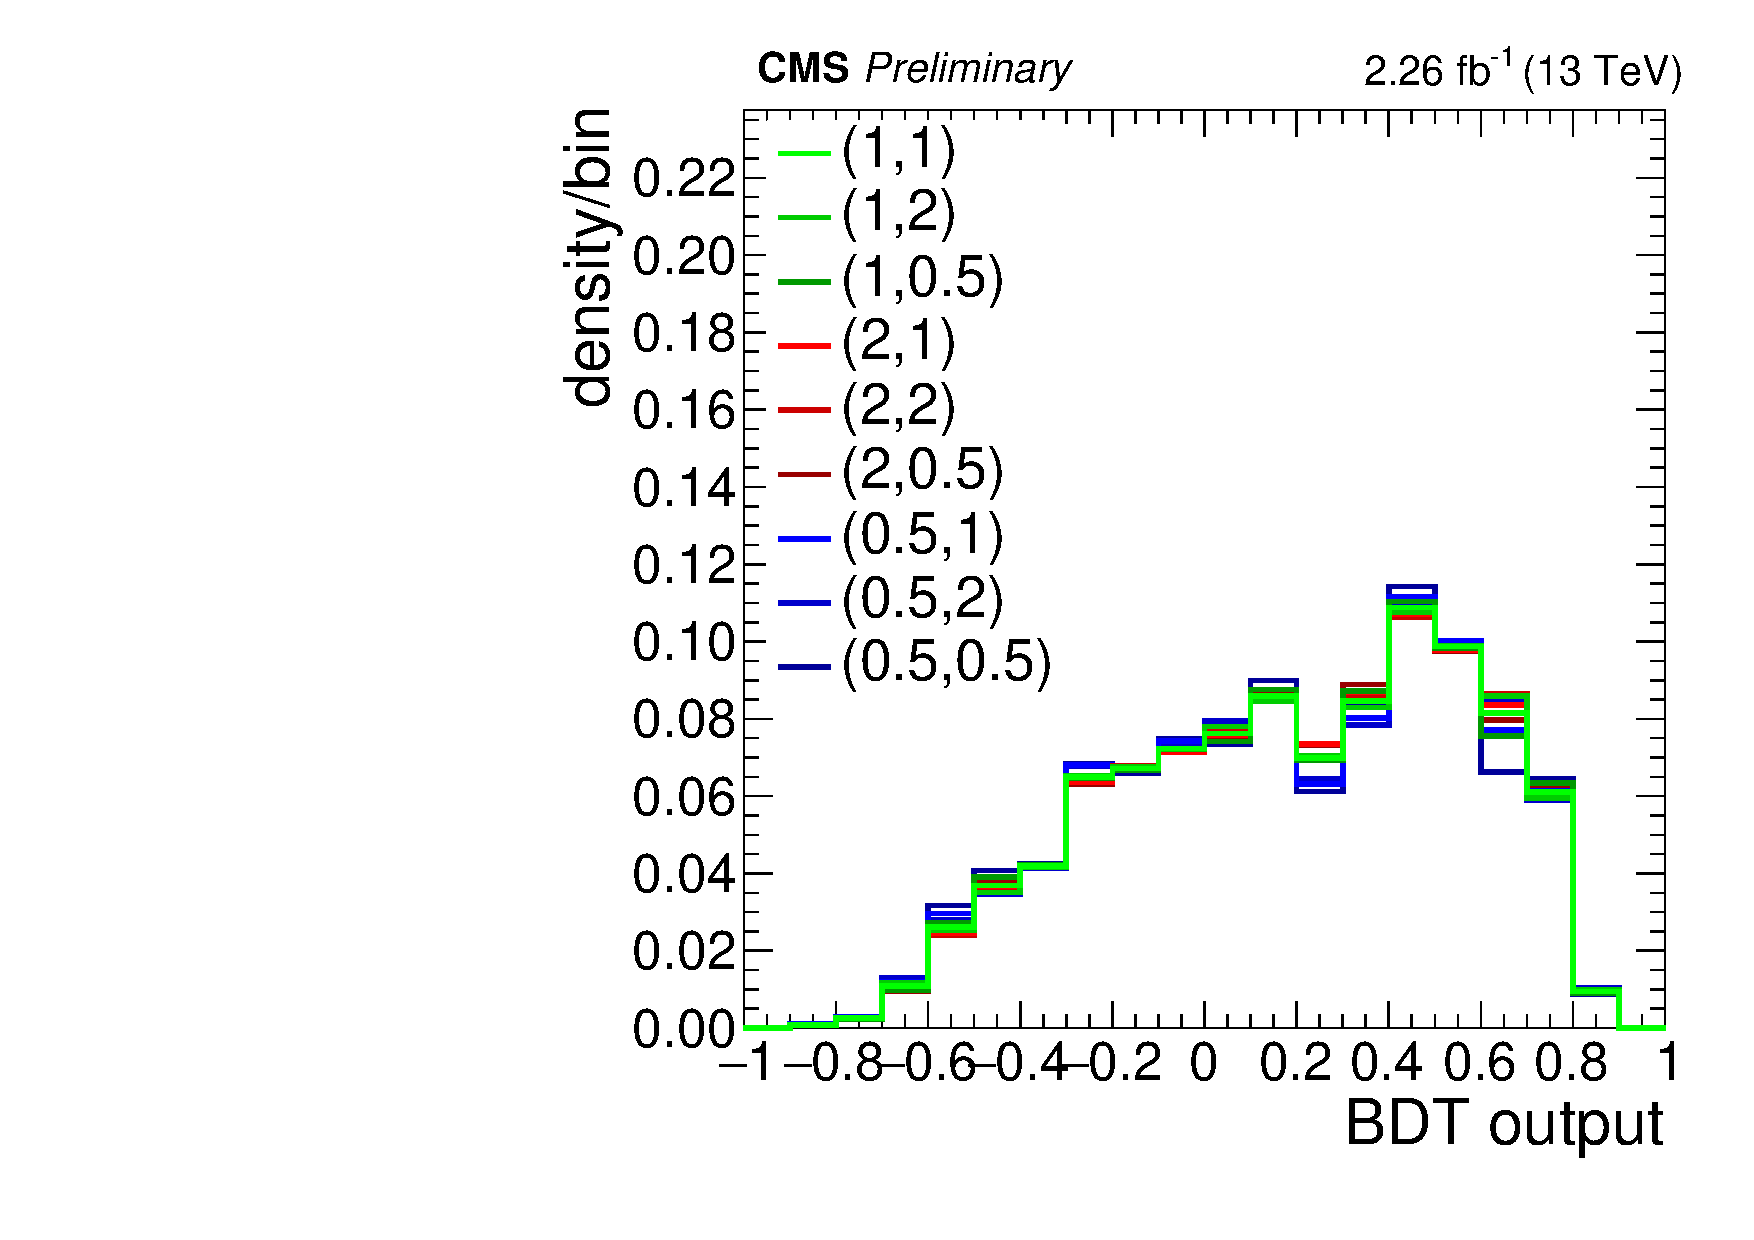
\includegraphics[width=0.35\textwidth]{plots_signal/theor_uncert/2lss/muR_muF_ttH/kinMVA_2lss_ttV}
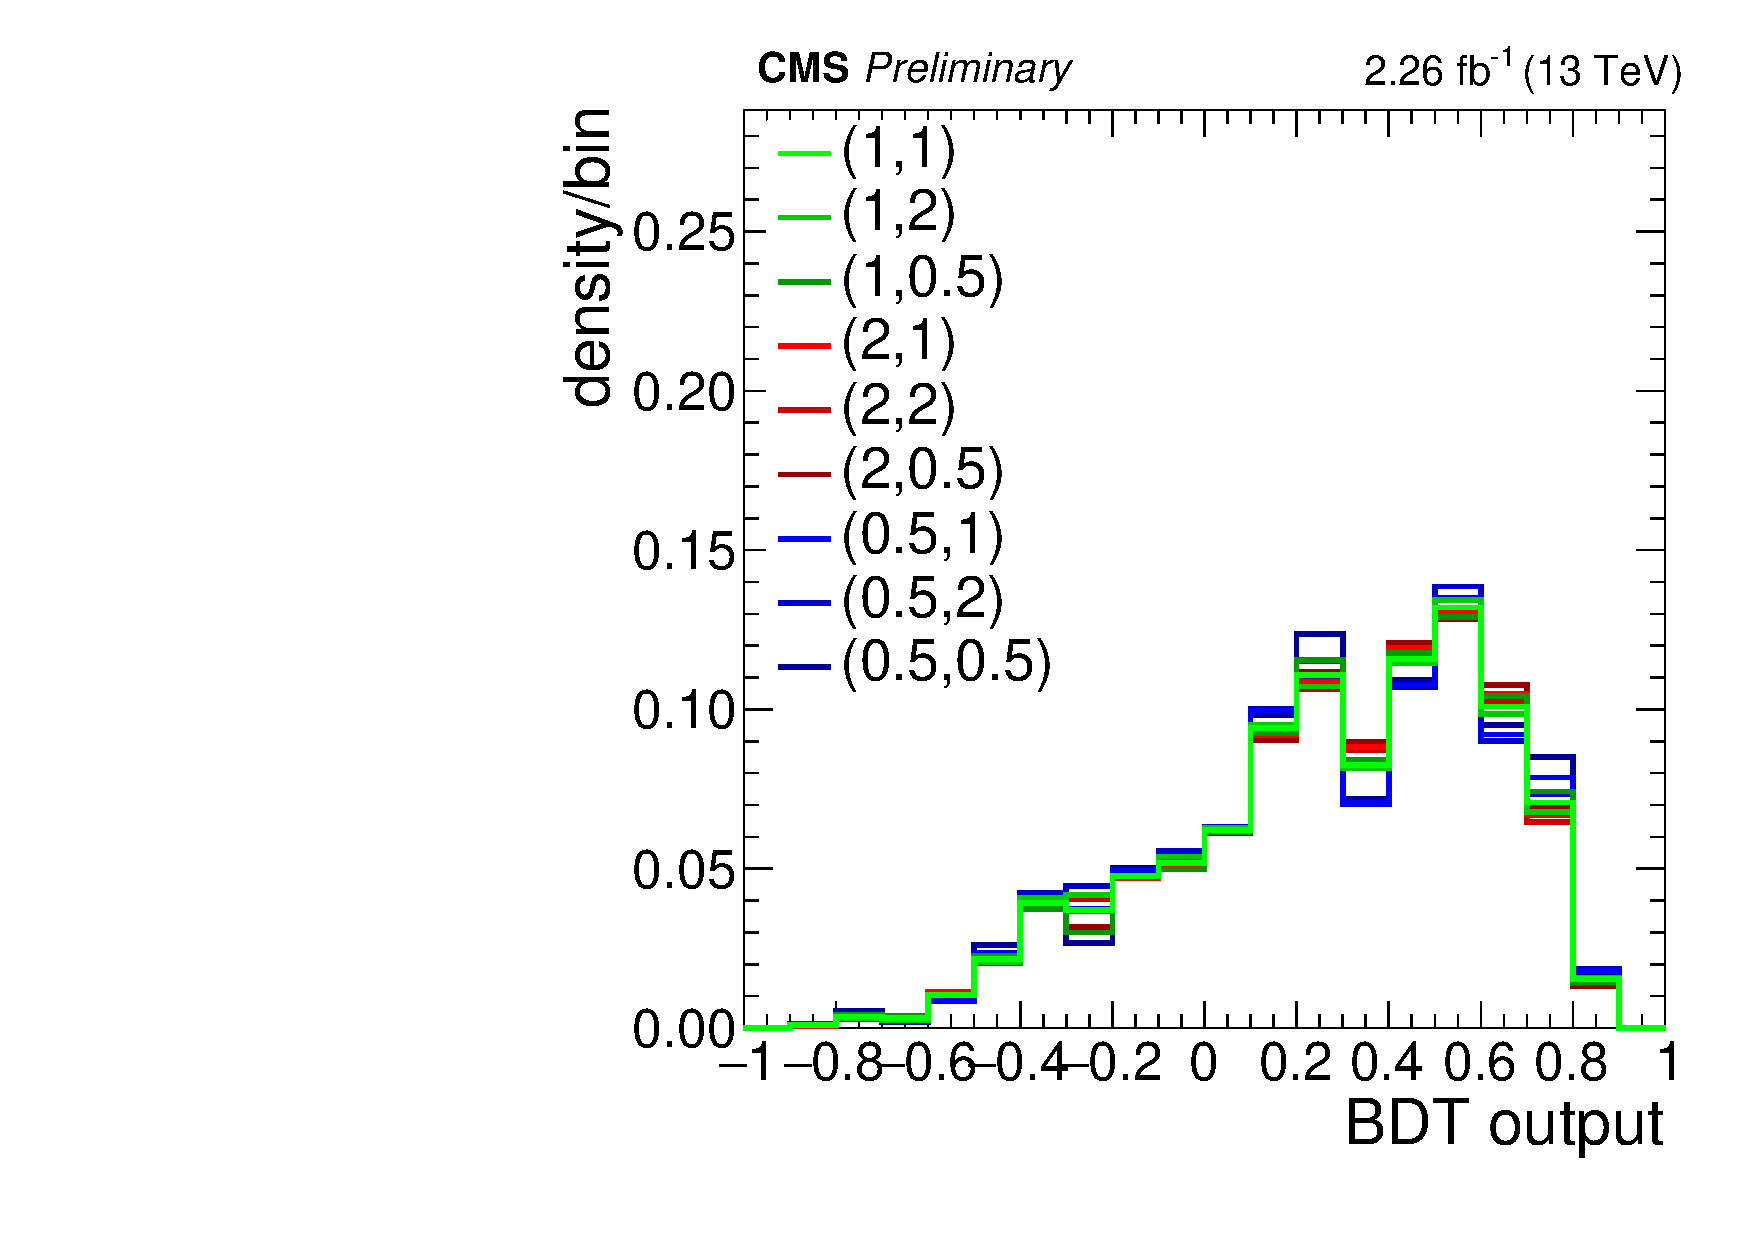
\includegraphics[width=0.35\textwidth]{plots_signal/theor_uncert/3l/muR_muF_ttH/kinMVA_3l_ttbar}
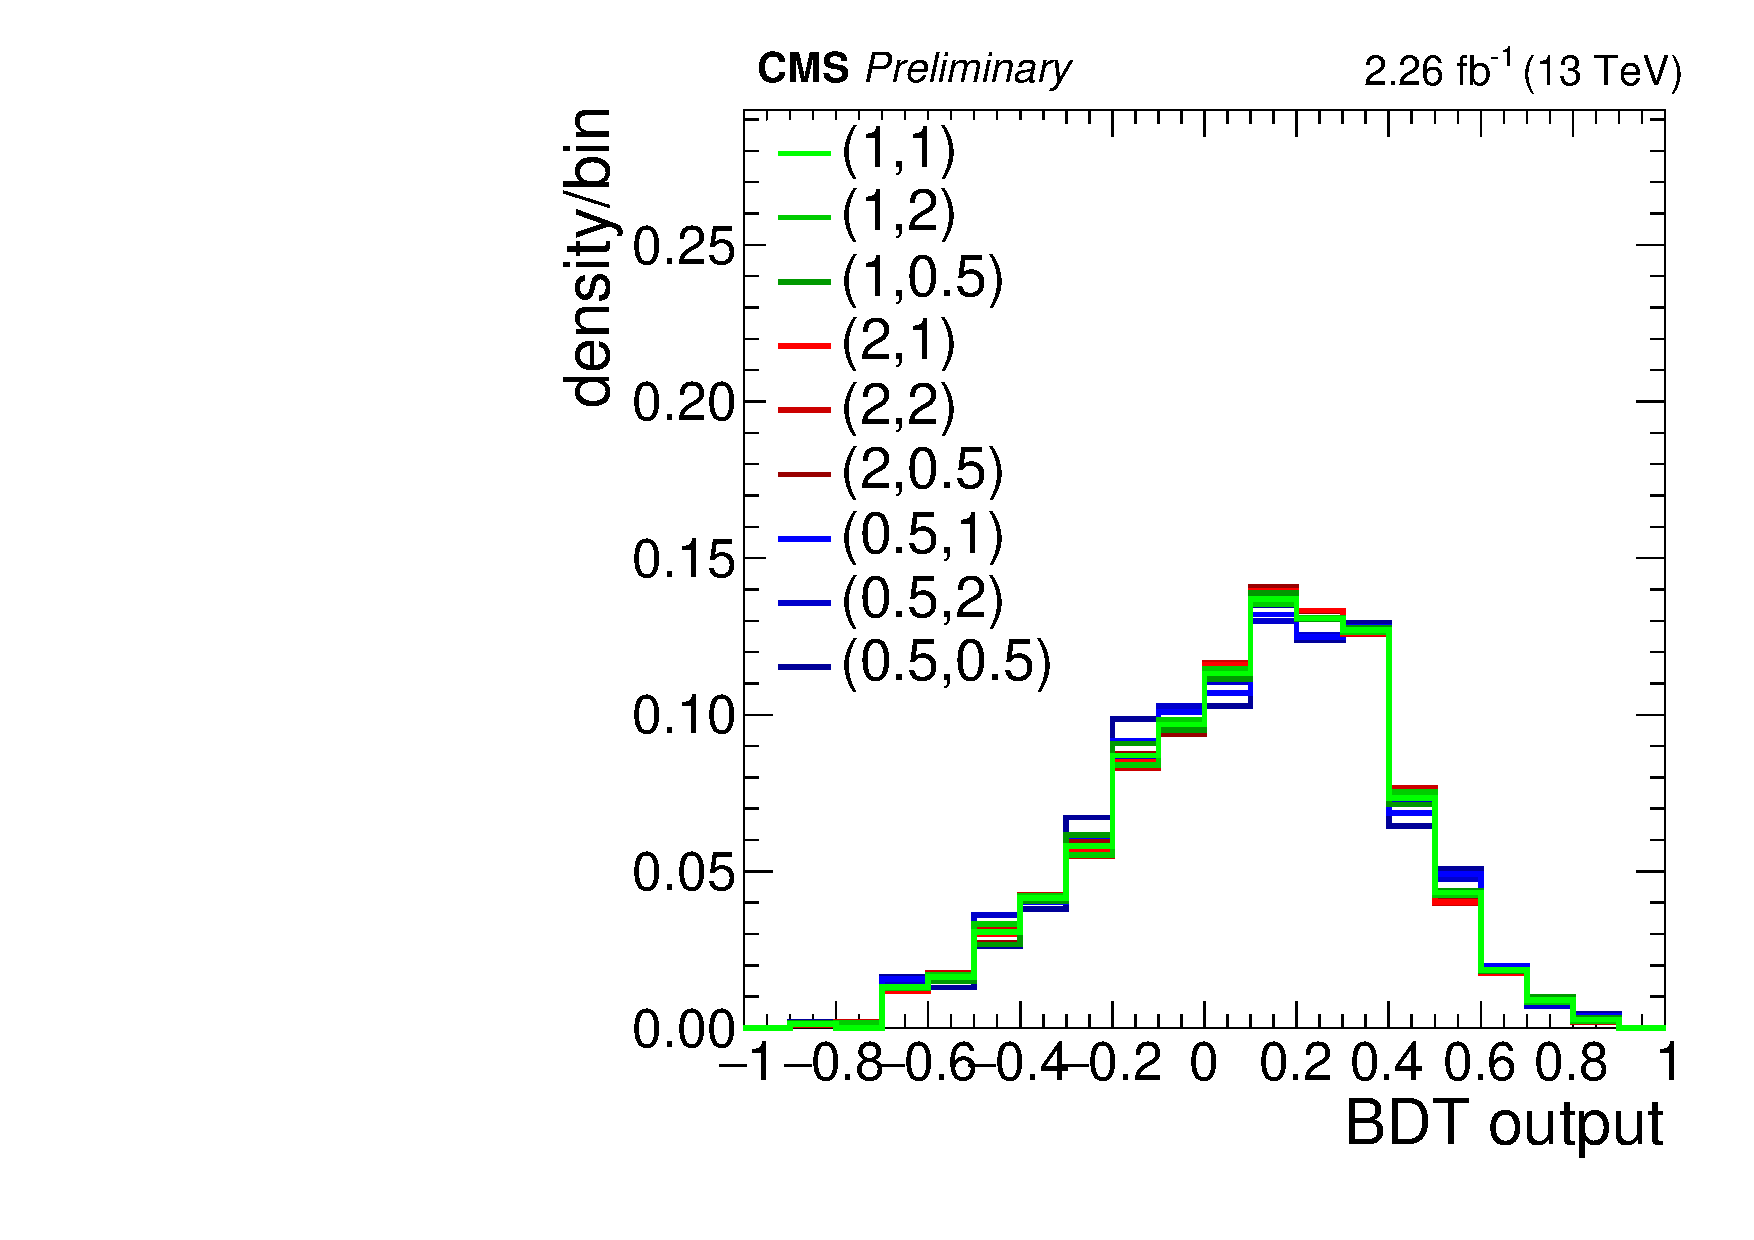
\includegraphics[width=0.35\textwidth]{plots_signal/theor_uncert/3l/muR_muF_ttH/kinMVA_3l_ttV}
	\caption{The BDT output distribution of the ttH signal, shown for the training against ttbar 
	(left) and ttV (right) in the two same sign leptons (upper) and three lepton (lower) final state, 
	with variations of the renormalization and factorization scale included in order to estimate the 
	shape uncertainties.}
	\label{fig:ScaleonBDTshape}
\end{figure}

